\newcommand{\OverviewofthePreviousIcarSystem}{
    asd asd asd asd asd asd asd asd    
    lorem ipsum dolor sit amet, consectetur adipiscing elit, sed do eiusmod tempor incididunt ut labore et dolore magna aliqua. Ut enim ad minim veniam, quis nostrud exercitation ullamco laboris nisi ut aliquip ex ea commodo consequat. Duis aute irure dolor in reprehenderit in voluptate velit esse cillum dolore eu fugiat nulla pariatur. Excepteur sint occaecat cupidatat non proident, sunt in culpa qui officia deserunt mollit anim id est laborum.
}

\newcommand{\OverviewoftheProposedSystem}{
    asd asd asd asd asd asd asd asd    
    lorem ipsum dolor sit amet, consectetur adipiscing elit, sed do eiusmod tempor incididunt ut labore et dolore magna aliqua. Ut enim ad minim veniam, quis nostrud exercitation ullamco laboris nisi ut aliquip ex ea commodo consequat. Duis aute irure dolor in reprehenderit in voluptate velit esse cillum dolore eu fugiat nulla pariatur. Excepteur sint occaecat cupidatat non proident, sunt in culpa qui officia deserunt mollit anim id est laborum.
}

\newcommand{\ElectricalSystem}{
    The Electrical System of Icar consists of two main subsystems: the Sensor System and the Actuation System. The Sensor System is responsible for gathering data from the environment and the vehicle itself, while the Actuation System controls the movement and operation of the vehicle based on the calculated data.
}

\newcommand{\SensorSystem}{
    \begin{figure}[H]
        \centering
        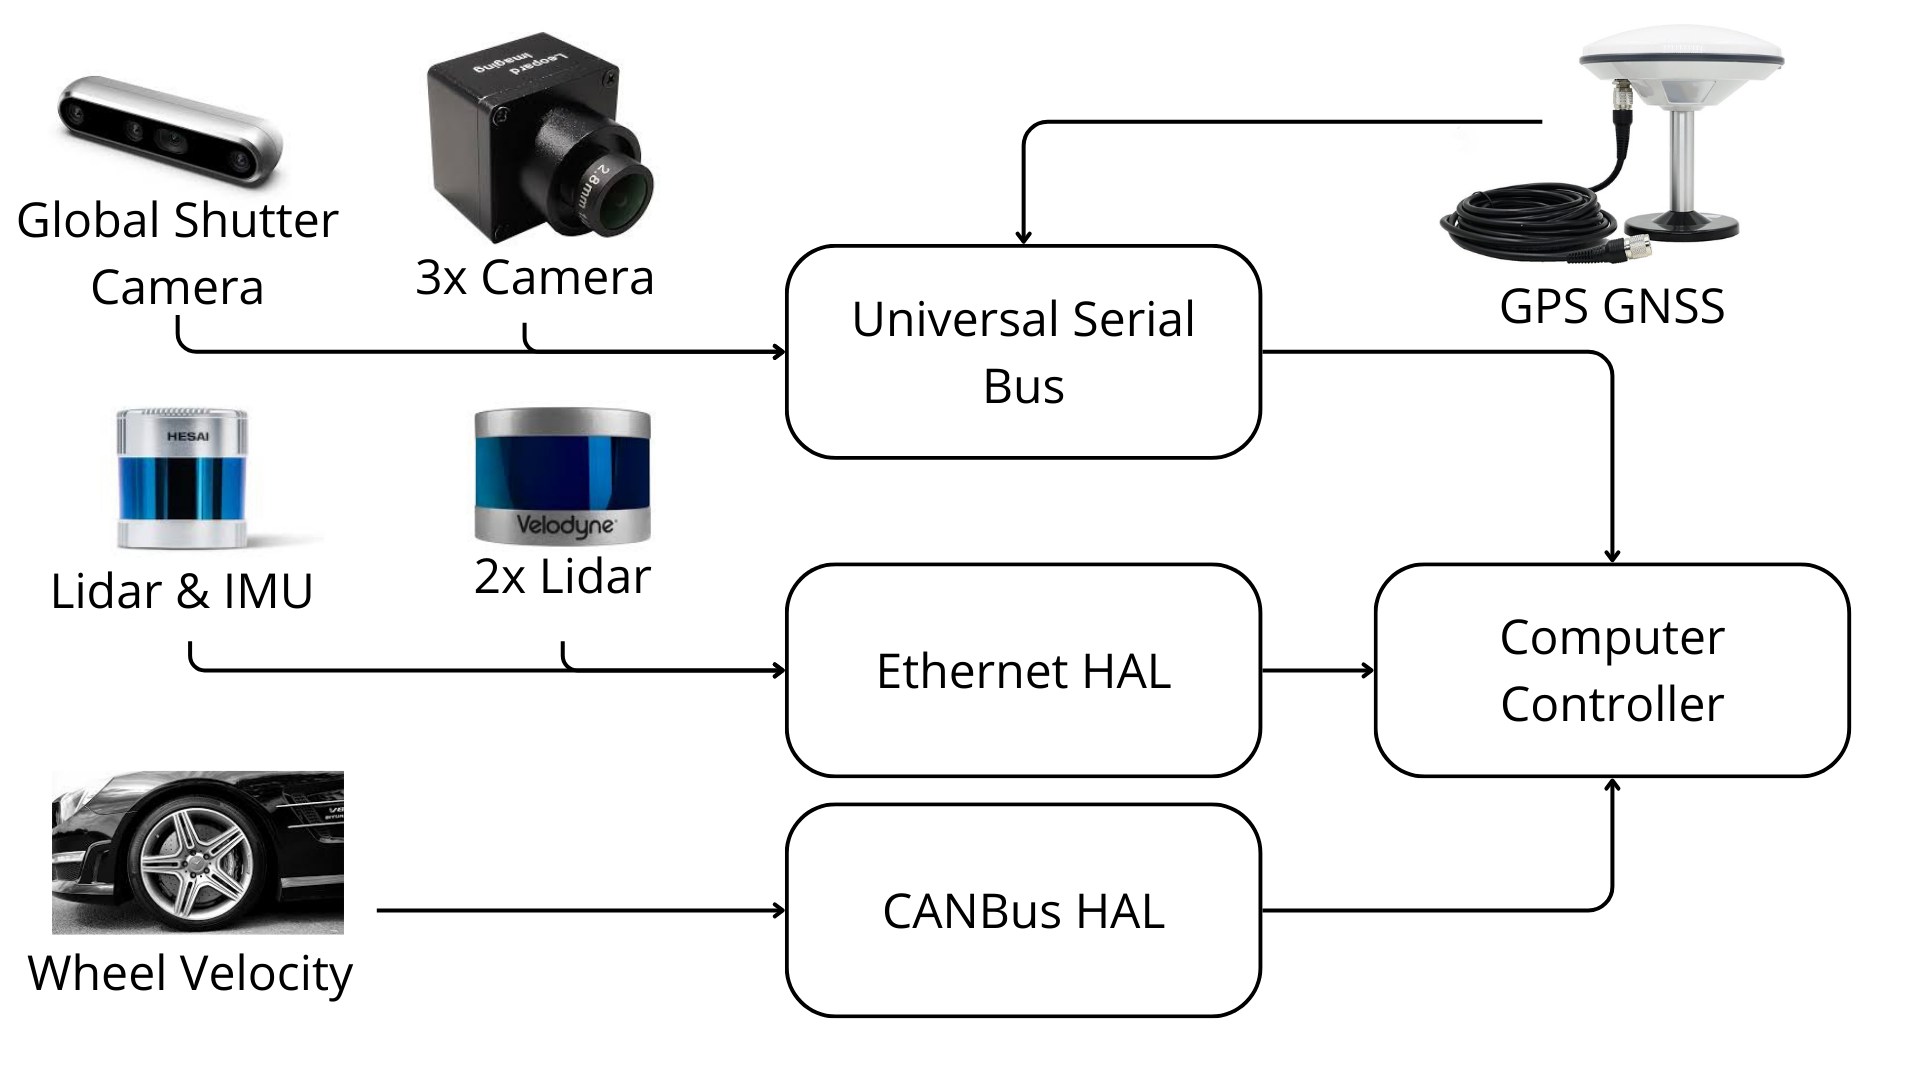
\includegraphics[width=\linewidth]{../konten/e_sensor_fix.png}
        \caption{Block Diagram of Sensor System}
        \label{fig:e_sensor}
    \end{figure}

    Based on Figure \ref{fig:e_sensor}, the Sensor System consists of several components, including LIDAR, Camera, GPS, and Wheel Velocity Sensor. The LIDAR sensors produces point cloud data and IMU data that interfaced with ethernet controller of computer. The Camera sensors produces image data that will be used for road segmentation, interfaced using USB controller of computer. The GPS sensor produces the estimation of latitude and longitude for car that interfaced using USB. The Wheel Velocity Sensor captured by sniffing car's main CAN bus using CANbus HAL module. 
}

\newcommand{\ActuationSystem}{
    \begin{figure}[H]
        \centering
        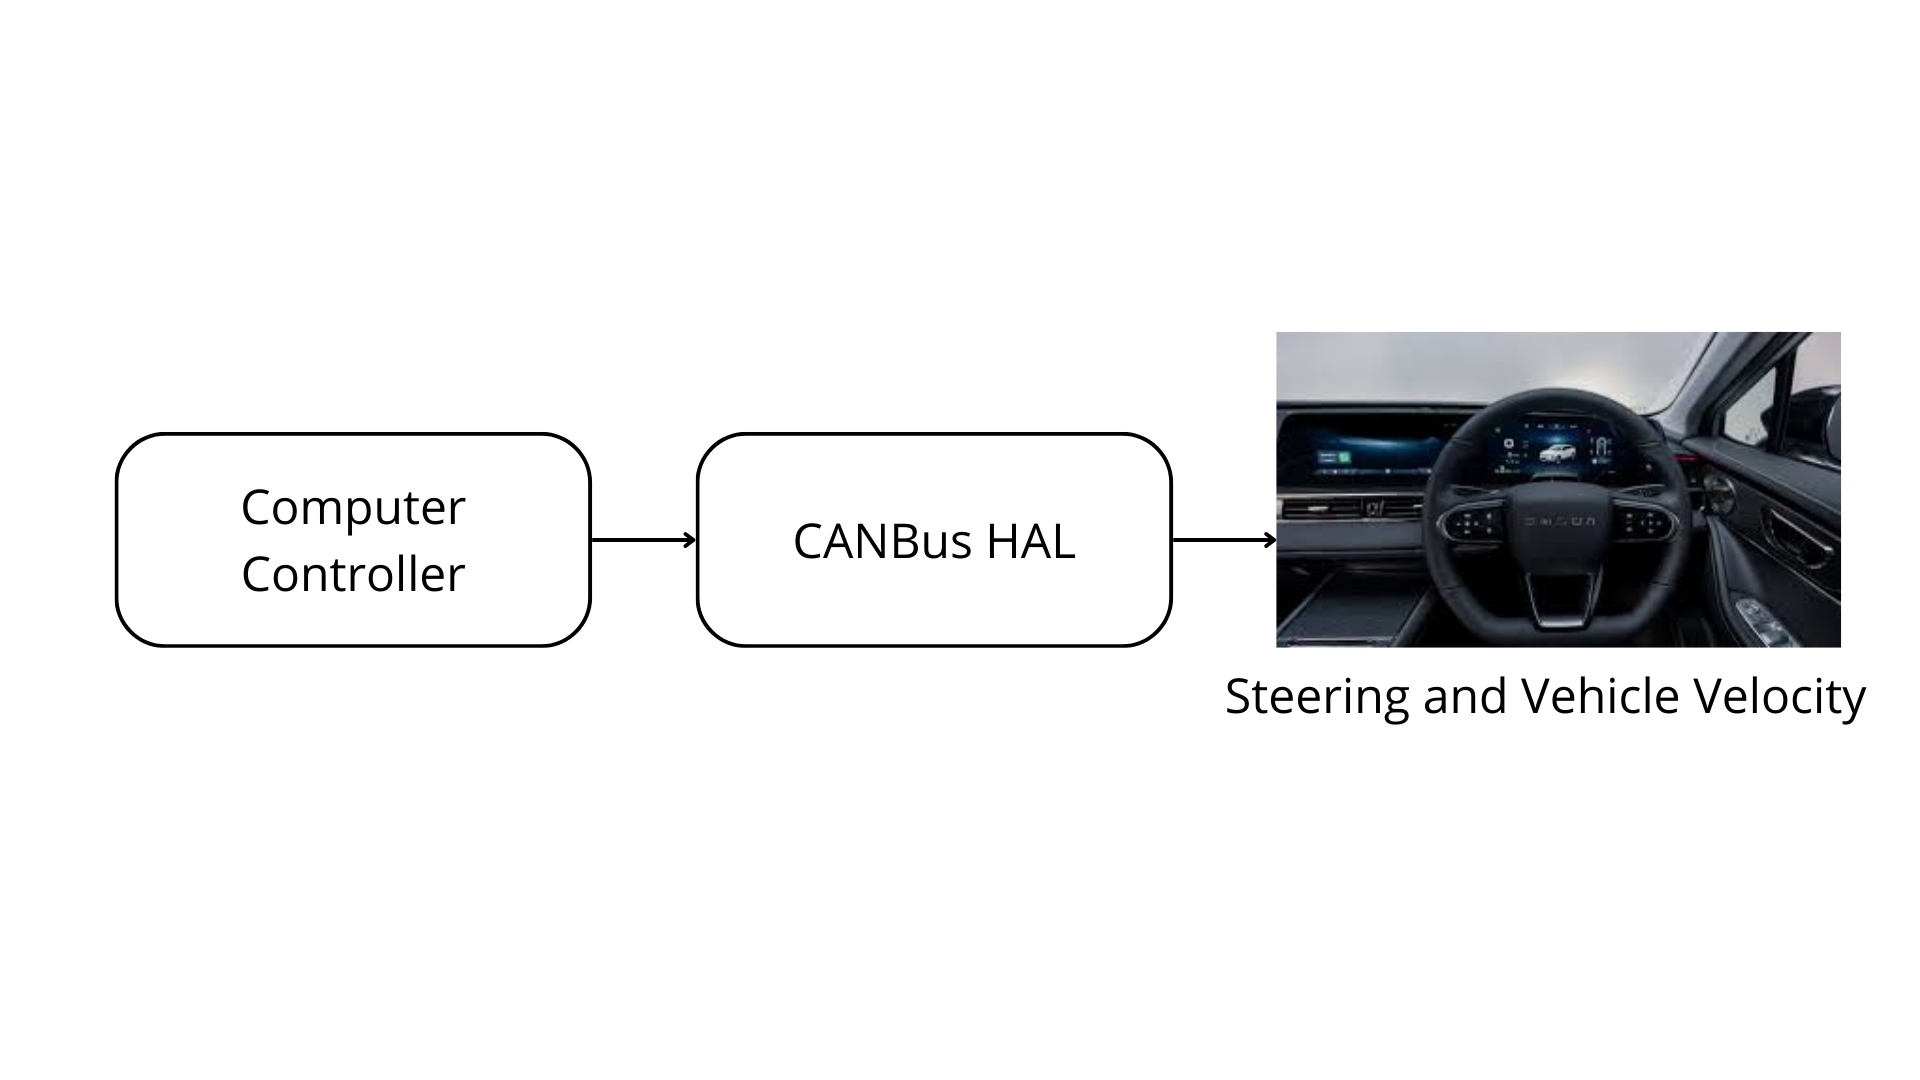
\includegraphics[width=\linewidth]{../konten/e_aktuator.png}
        \caption{Block Diagram of Actuation System}
        \label{fig:e_aktuator}
    \end{figure}

    Based on Figure \ref{fig:e_aktuator}, the Actuation System only proceeds Steering Angle and Velocity of vehicle. The commands are sent from the car's main CAN bus using CANbus HAL module. That technique is called Drive by Wire (DBW), where there is no physical connection between the driver and the actuator. The commands are generated using electrical signals from the computer to the car's main CAN bus.
}

\newcommand{\Limitations}{
    The limitations of the system are divided into two main categories: Sensor Limitations and Actuation Limitations. Each category has its own set of challenges that need to be addressed to ensure optimal performance of the autonomous vehicle.
}

\newcommand{\SensorLimitations}{
    There are several limitations associated with the sensors used in the system. The limitations listed below: 
    \begin{itemize}
        \item The noise measurement of GPS that can reach up to 2.5 meters in open sky condition, and can be worse in urban area with tall buildings or trees that can block the satellite signal.
        \item LIDAR Point Cloud has update rate limitation from 5 Hz to 20 HZ, which may affect the real-time performance for the higher level of system. 
        \item There is 30 cm blindspot in front of car because of Lidar and Camera Mounting.
    \end{itemize}
}

\newcommand{\ActuationLimitations}{
    There are several limitations associated with the actuation system used in the vehicle. The limitations listed below:
    \begin{itemize}
        \item The maximum car acceleration is \(3.0\,\text{m/s}^2\) based on ISO 11270, which limits the speed of response for velocity control. 
        \item The maximum steering angle rate is \(5\,\text{deg/s}\) based on car's specification, which limits the speed of response for steering control. 
        \item The maximum steering angle position is \(\pm 300\,\text{deg}\) based on car's specification, which limits the turning radius of the vehicle.
    \end{itemize}
}

\newcommand{\LowLevelProgramArchitecture}{
    \begin{figure}[H]
        \centering
        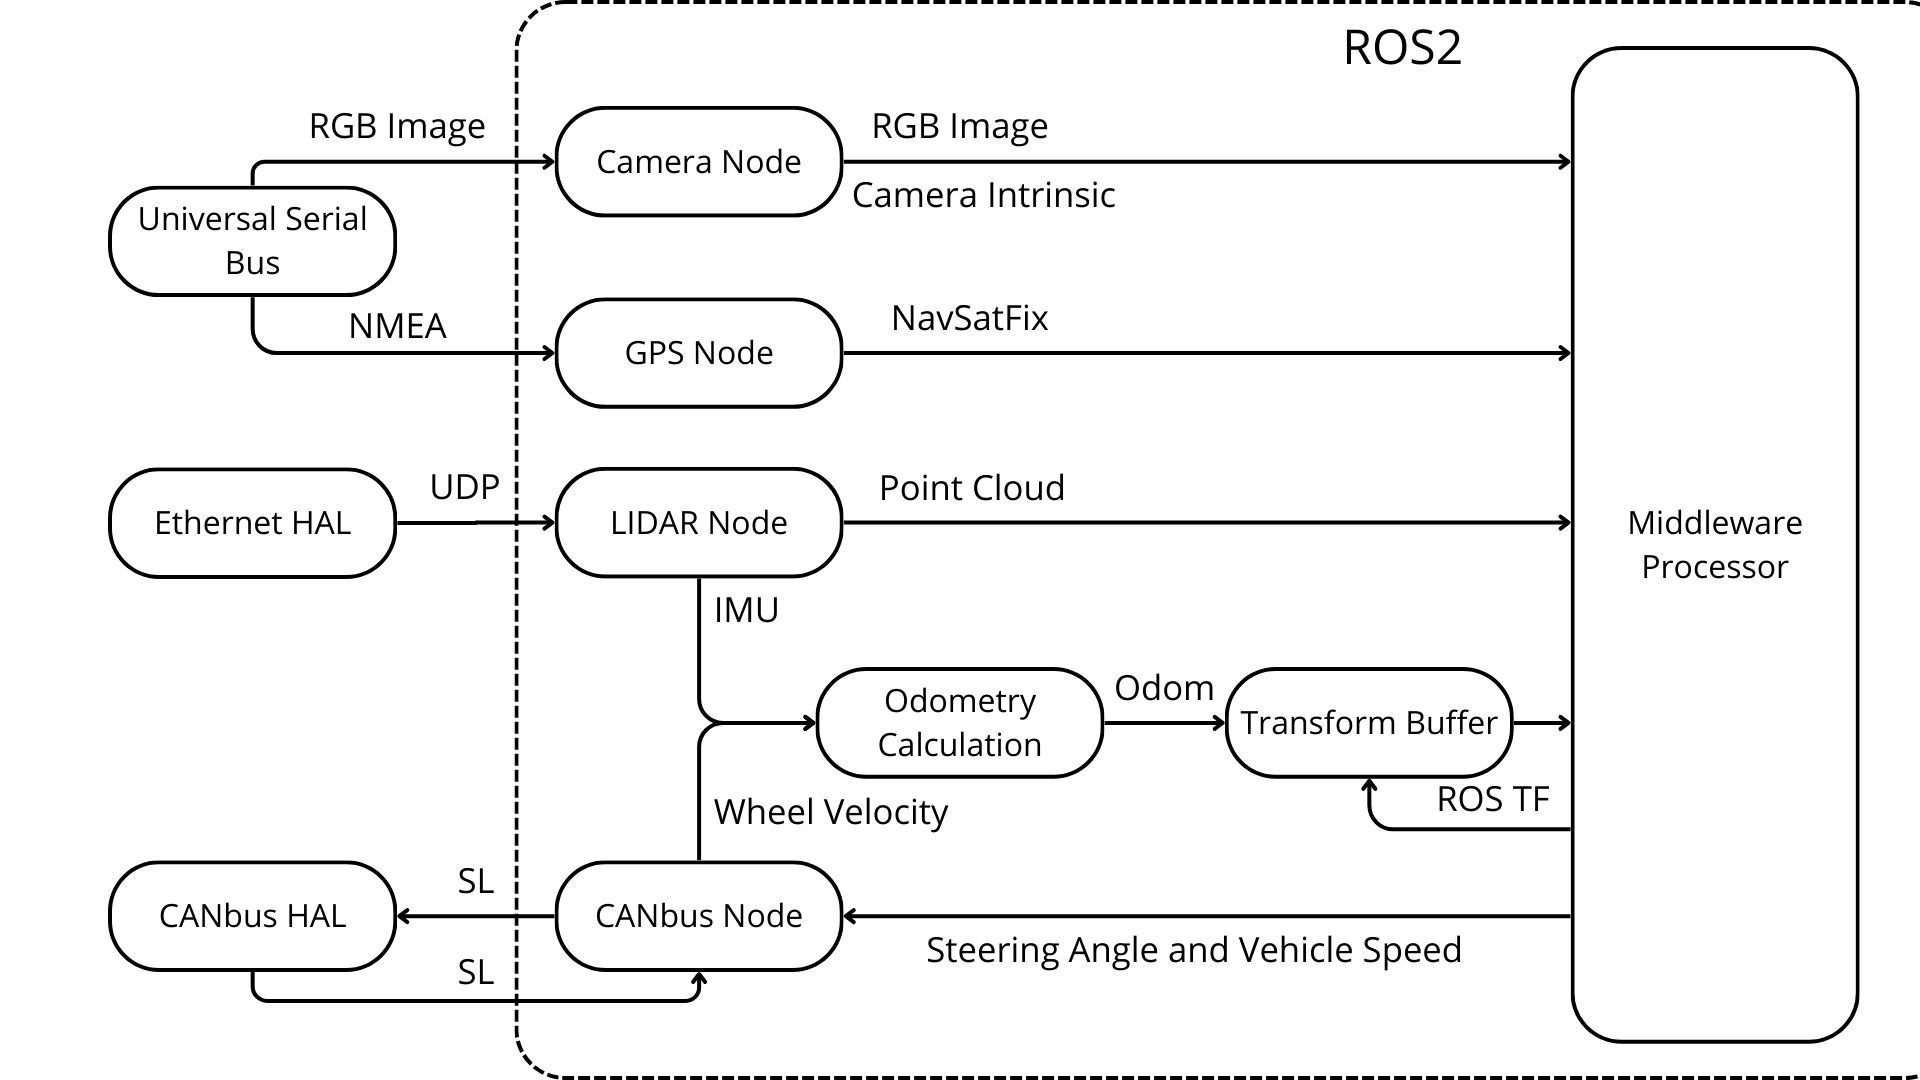
\includegraphics[width=\linewidth]{../konten/low_system_fix.png}
        \caption{Block Diagram of Low Level Architecture}
        \label{fig:low_level_arc}
    \end{figure}
    Based on Figure \ref{fig:low_level_arc}, the Low Level Program Architecture utilizes ROS2 as the framework for all processes. There are three main parts of Low Level Architecture, which are Sensor Data Acquisition, Odometry Calculation, and Frame Transformation. 
}

\newcommand{\SensorDataAcquisition}{%
    Based on Figure~\ref{fig:low_level_arc}, the Sensor Data Acquisition block is responsible for acquiring raw data from the LIDAR, camera, GPS, and wheel velocity sensor. For each sensor, we have a single independent ROS~2 node that publishes a standard ROS~2 message type. We use several standard ROS~2 message types in this part, such as \texttt{sensor\_msgs/PointCloud2} for LIDAR point cloud data, \texttt{sensor\_msgs/Image} for camera image data, \texttt{sensor\_msgs/NavSatFix} for GPS data, and \texttt{std\_msgs/Float32} for wheel velocity data.%
}

\newcommand{\FrameTransformation}{%
    Based on Figure~\ref{fig:low_level_arc}, there is a step called the transformation buffer. This part is responsible for managing the transformations between each sensor frame and the main frames, such as \texttt{base\_link}, \texttt{odom}, and \texttt{map}. The diagram of the transformations between each frame is shown in Figure~\ref{fig:tf_buffer}.

    \begin{figure}[H] 
        \centering
        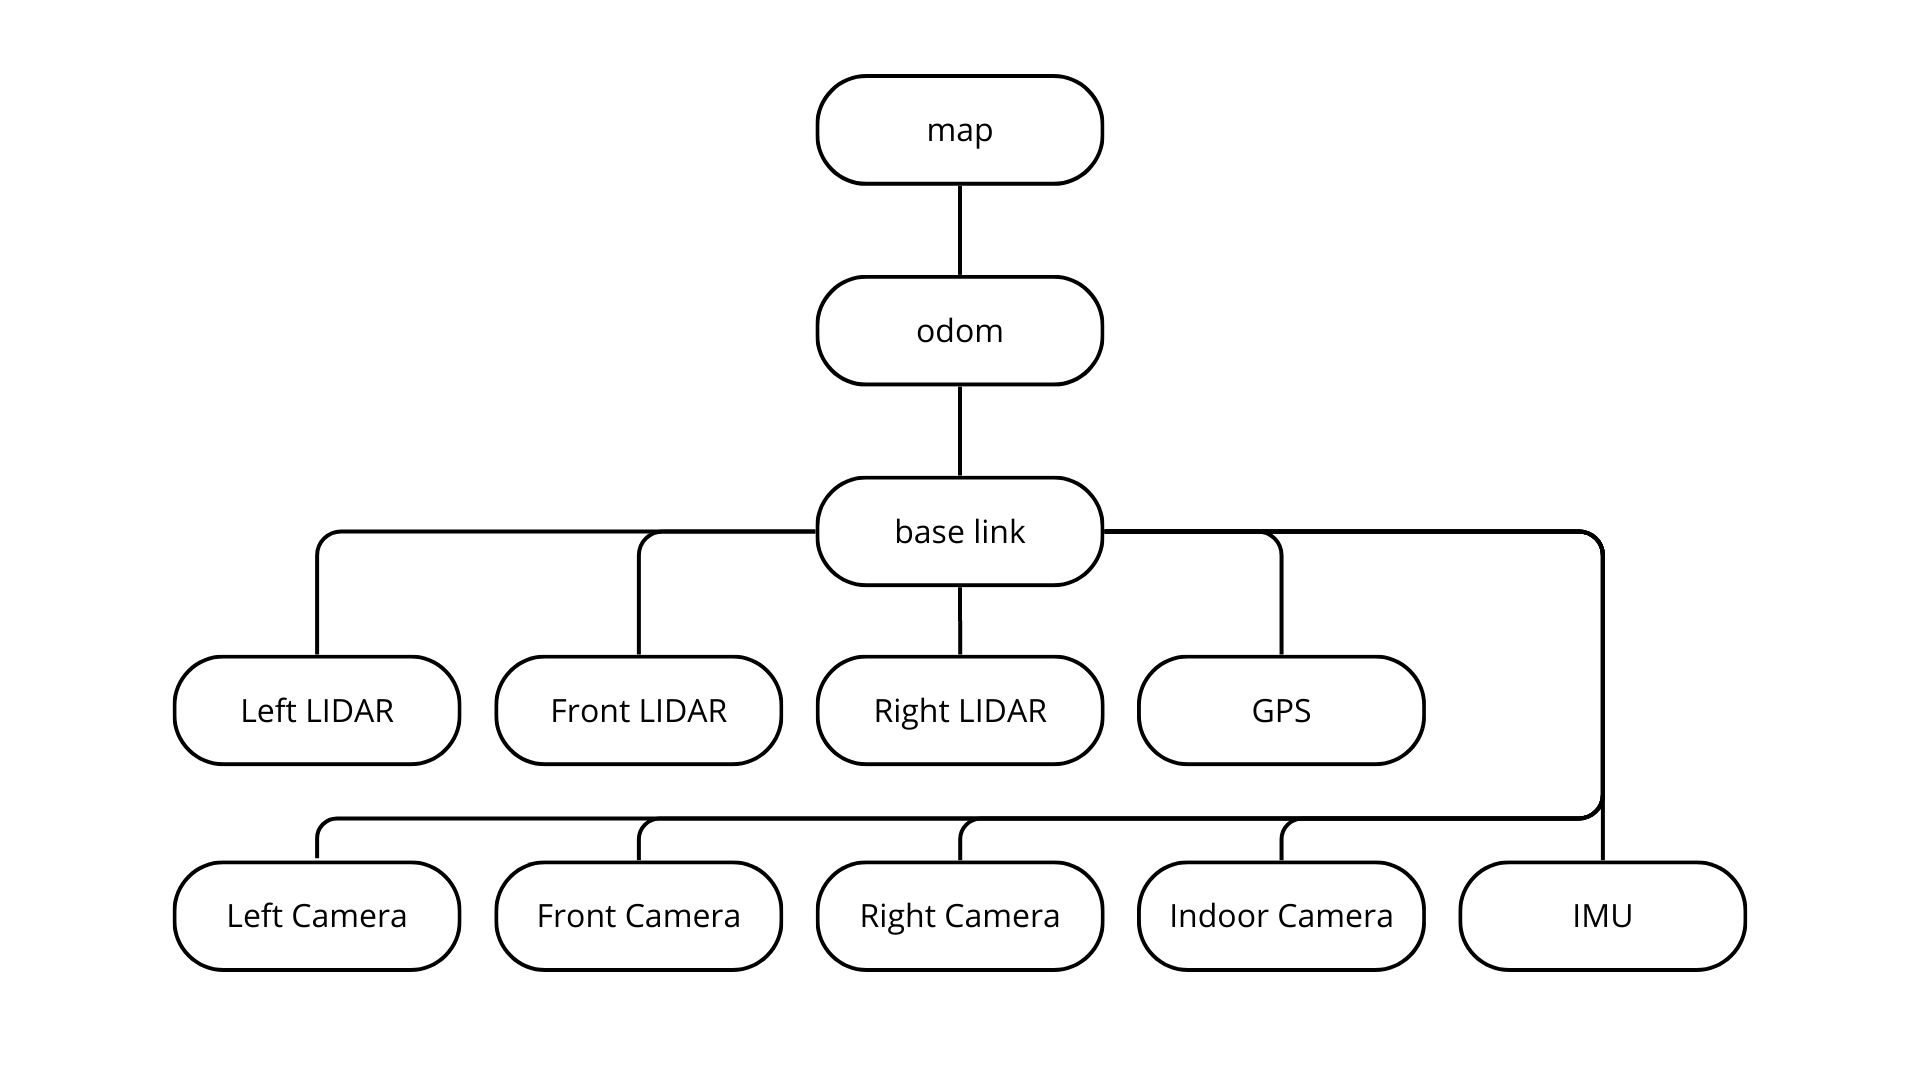
\includegraphics[width=\linewidth]{../konten/tf_tree.png}
        \caption{Transformation buffer}
        \label{fig:tf_buffer}
    \end{figure}

    Figure~\ref{fig:tf_buffer} shows the transformations between each frame. The \texttt{base\_link} frame is the main frame of the vehicle, which is located at the center of the vehicle. The \texttt{odom} frame represents the odometry, which is calculated from the wheel velocity sensor and IMU data from the LIDAR. The \texttt{map} frame is the global world frame that represents the global position of the vehicle. The transformations between frames are managed using the \texttt{tf2} library in ROS~2.%
}

\newcommand{\OdometryCalculation}{%
    Based on Figure~\ref{fig:low_level_arc}, the next step after Sensor Data Acquisition is Odometry Calculation. This block is responsible for computing the odometry from the wheel velocity sensor and the IMU data from the LIDAR. The odometry is calculated using a differential-drive kinematic model, which takes into account the wheel velocities and the time interval between measurements. The resulting odometry data is then published as a \texttt{nav\_msgs/Odometry} message type.%
}

\newcommand{\MiddlewareSystem}{
    \begin{figure}[H] 
        \centering
        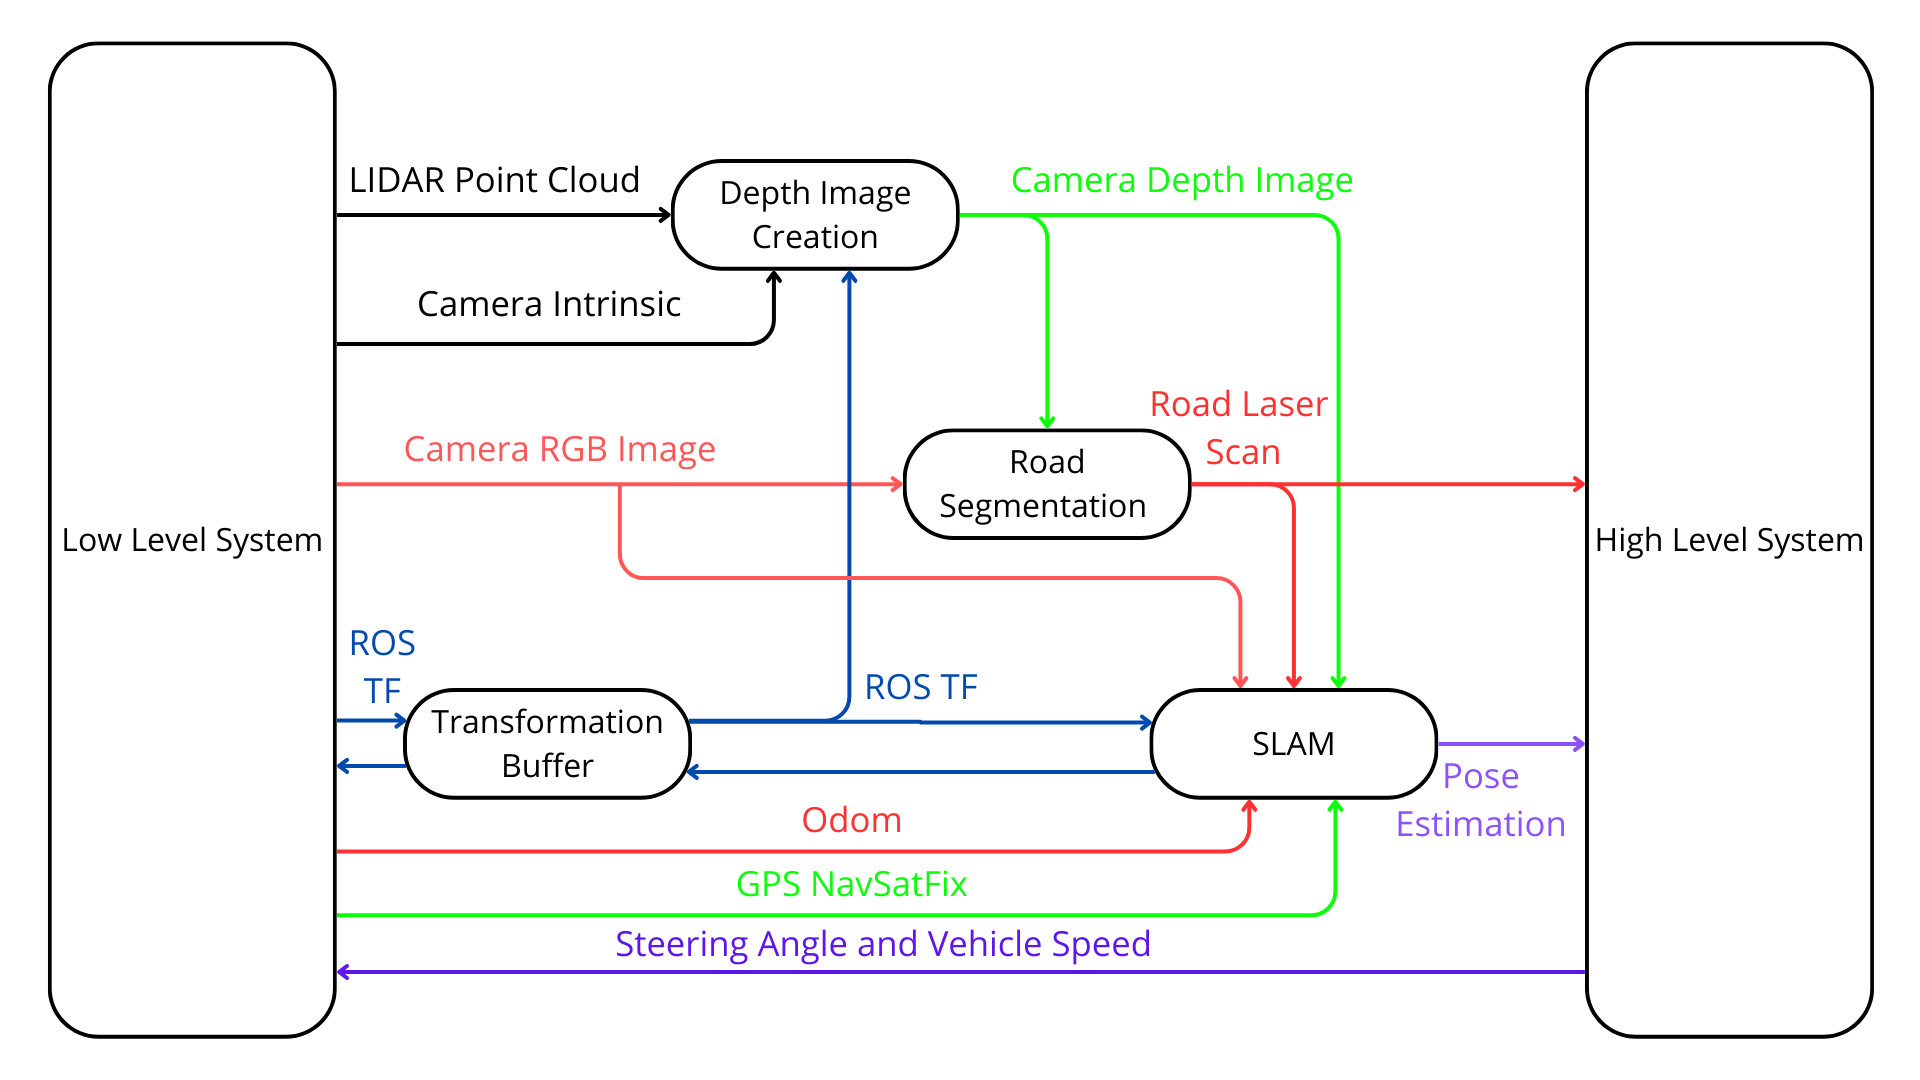
\includegraphics[width=\linewidth]{../konten/middleware_fix_coy.png}
        \caption{Block Diagram of Middleware System}
        \label{fig:middleware_system}
    \end{figure}

    Figure \ref{fig:middleware_system} shows the Middleware System that connects the Low Level Program Architecture with the High Level Program Architecture. There are three main parts in Middleware System, the first part is the Depth Image Creation, the second part is Road Segmentation using Machine Learning, and the third part is Graph Based SLAM for Pose Correction and Estimation.
}

\newcommand{\DepthImageCreation}{
    \label{sec:depth_image_creation}
    Base on Figure \ref{fig:middleware_system}, the Depth Image Creation block is responsible for creating a depth image from the LIDAR point cloud data and camera intrinsic data. This process involves two main steps: LIDAR Concatenation and Post Filter for Depth Image.
}

\newcommand{\LIDARConcatenation}{
    \label{sec:lidar_concat}
    LIDAR Concatenation is the process of combining multiple LIDAR scans into a single point cloud. This is done to increase the density of the point cloud and improve the accuracy of the depth image. The concatenated point cloud is then projected onto the camera optical frame. The transformation lookup between the LIDAR frame and the camera frame can be obtained from the transformation buffer in the Low Level Program Architecture \ref{fig:tf_buffer}.   

    \par   
    After transformed point cloud to the camera optical frame, we can calculate the depth image using the camera intrinsic parameters. Each point in the point cloud is projected onto the image plane using the pinhole camera model, and the depth value is calculated based on the distance from the camera to the point. 
}

\newcommand{\PostFilterForDepthImage}{
    The raw depth image obtained from the previous step has some hole areas due to the sparse nature of the LIDAR point cloud. To address this issue, a post-filtering process is applied to fill in the holes and smooth the depth image. This process involves using morphological operations to fill in the holes by neighboring pixel values.
}

\newcommand{\MachineLearning}{
    Based on figure \ref{fig:middleware_system}, another sub process of middleware is Road Segmentation. Road Segmentation is done using Machine Learning approach. The idea is to segment each pixel of the image into two classes, which are road and non-road. The segmentation result will be transformed base link frame using depth image from previous step. The output of this process is a laser scan msg that will be used by high level system to determine target velocity and steering angle.
}

\newcommand{\InfrastructureSetup}{
    asd asd asd asd asd asd asdasdasdasd
}

\newcommand{\ArchitectureDesign}{
    \begin{figure}[H] 
        \centering
        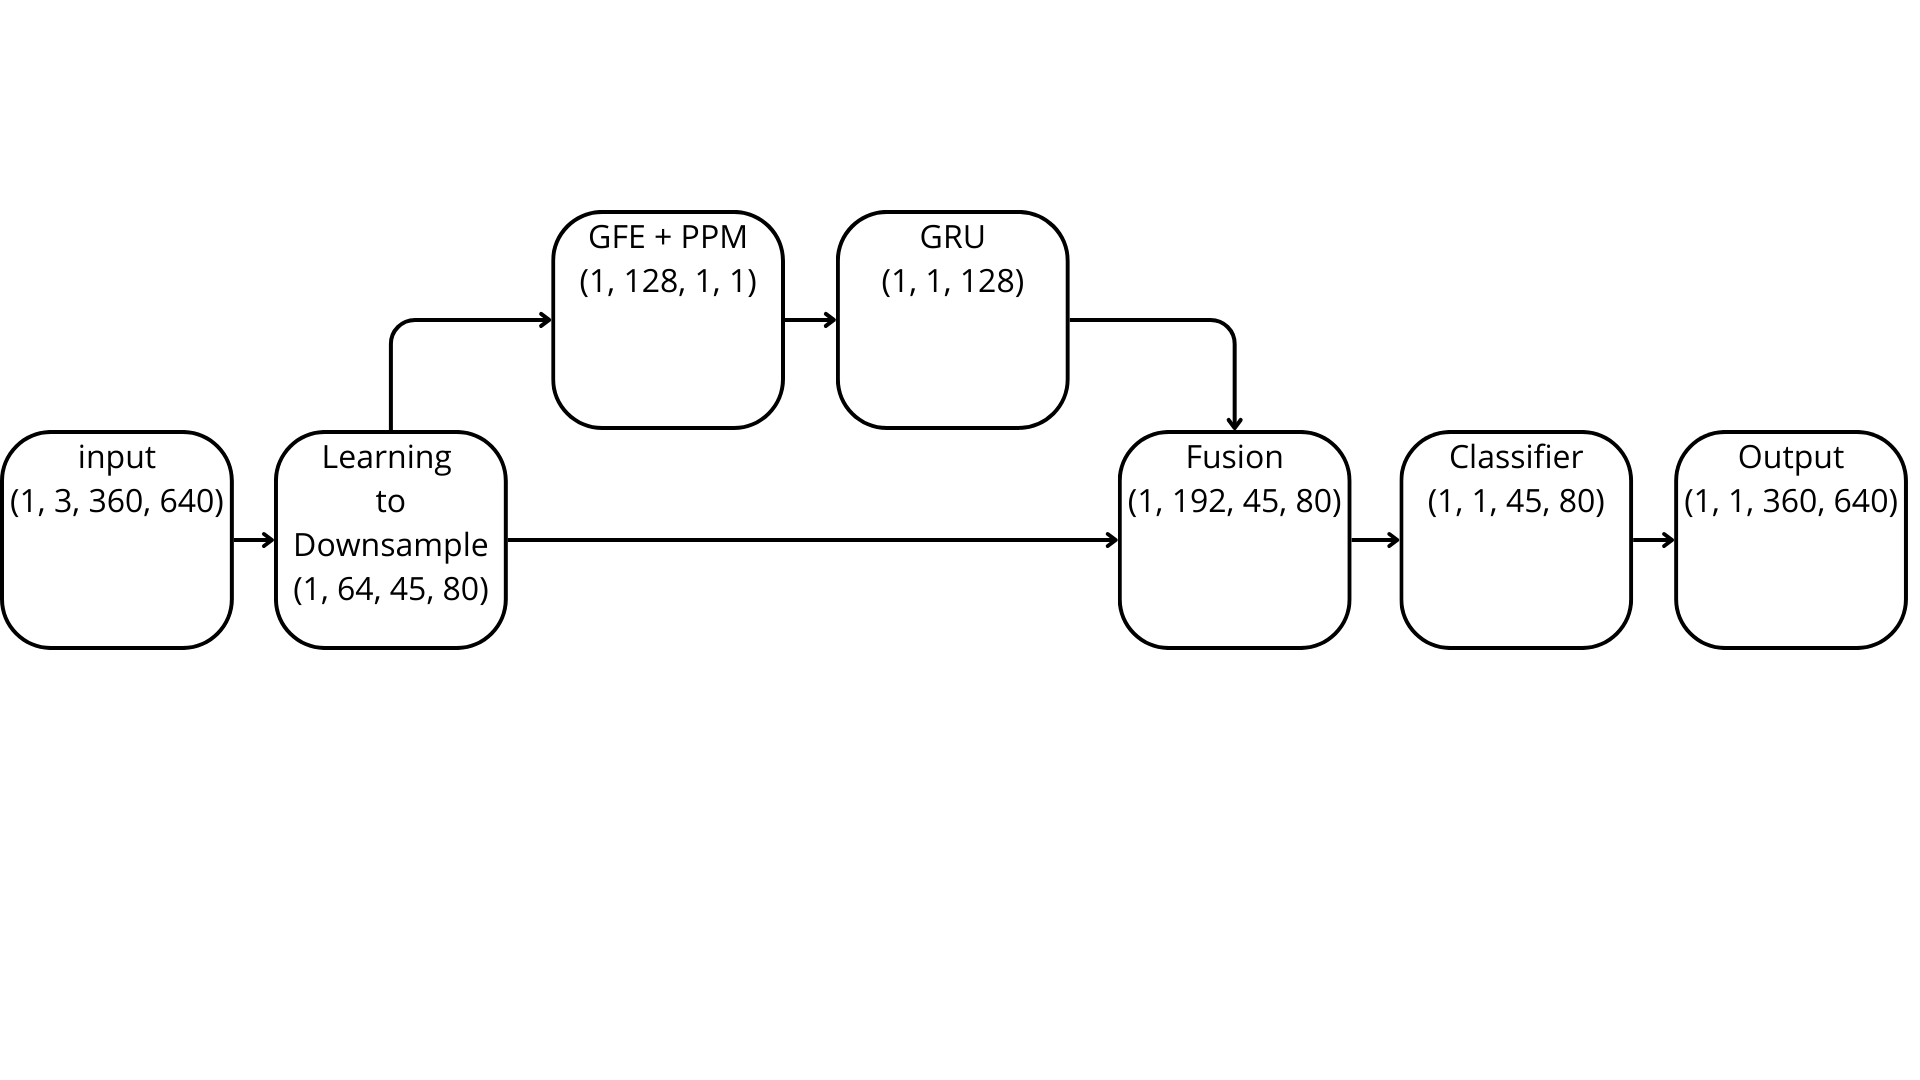
\includegraphics[width=\linewidth]{../konten/mlml.png}
        \caption{Machine Learning Architecture}
        \label{fig:ml_arch}
    \end{figure}

    Figure \ref{fig:ml_arch} visualize the architecture of our proposed new Machine Learning method. Based on Fast-SCNN, we proposed our new improvement method by adding GRU (Gated Recurrent Unit). The main idea of adding GRU to the existence of Fast-SCNN is to make a global context. That method can make the temporal effect on detection. 
}

\newcommand{\DatasetPreparation}{
    The preparation of dataset is crucial to Machine Learning process. The dataset only have one class called road class. The dataset image captured by driving the car through various road conditions, such as different lighting conditions, weather conditions, and road types. The dataset is then annotated manually to create ground truth labels for the road class. 
    
    \begin{figure}[H] 
        \centering
        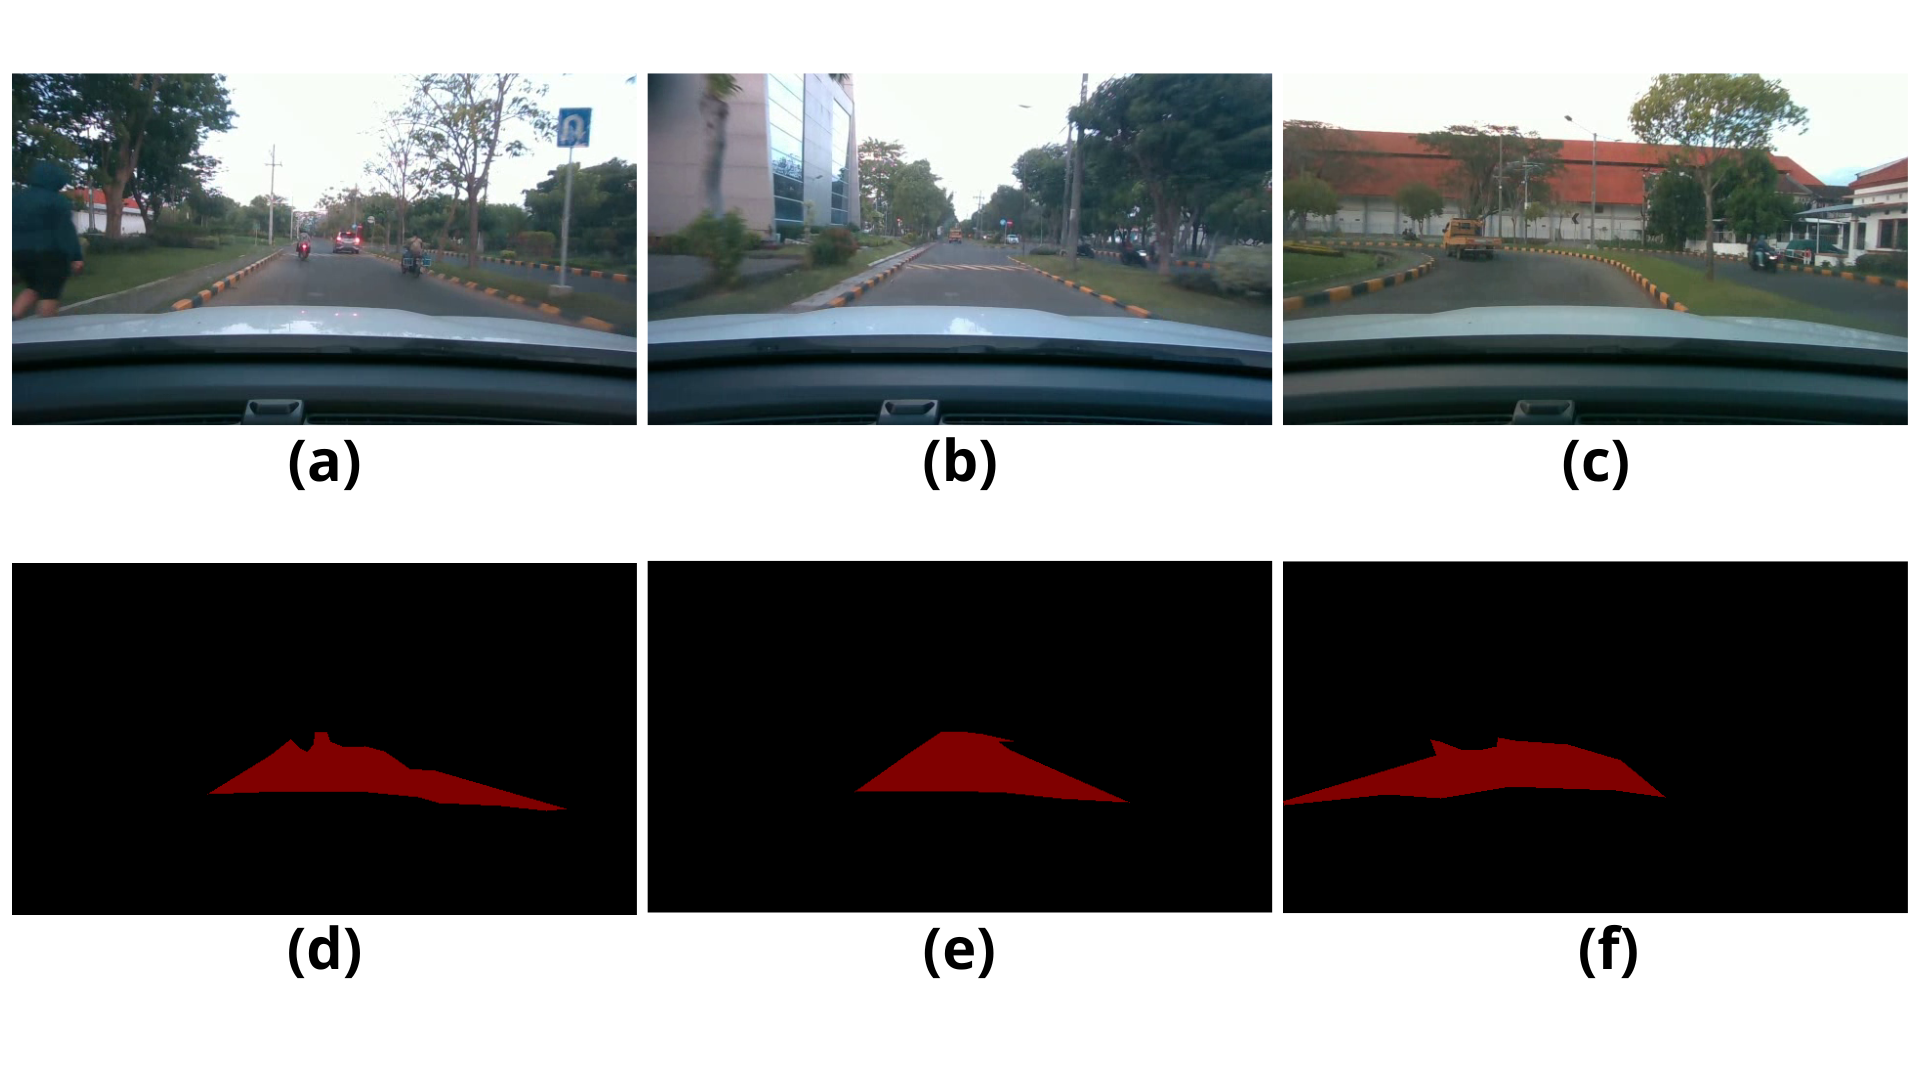
\includegraphics[width=\linewidth]{../konten/ml_dataset_fix.png}
        \caption{DAtasets for Machine Learning}
        \label{fig:ml_dataset}
    \end{figure}

    Figure \ref{fig:ml_dataset} shows some example of 1000 images dataset that we used for training and validation. The image a, b, and c are the rgb input image, while the image d, e, and f are the corresponding ground truth labels for road class. The red segmented area in the ground truth labels represents the road class. 
}

\newcommand{\ModelTraining}{
    The model training process is carried out using the prepared dataset. The problem of our dataset is imbalanced data for example on figure \ref{fig:ml_dataset} in sub image b, there is a road bumb that have same color and pattern with road barrier but we want to predict that it's a road too. To handle that imbalanced data we use the Tversky loss function during training. The Tversky loss function can handle imbalanced data and bunch of false positive cases \cite{ref_tversky}. The important of the bunch of false positive cases is to avoid the vehicle from misdetecting the road area as non-road area, which can lead to unsafe driving conditions. 
    \par    
    Another technique that we use to improve the model performance is data augmentation. Data augmentation is done by applying various transformations to the input images, such as random gamma, random brightness, CLAHE, HSV limit, RGB shift, random shadow, random sunflare, ISO noise, Motion blurr, random tone curve, and random brightness contrast. These transformations help to increase the diversity of the training data and improve the model's ability to generalize to unseen data.  
    \par     
    Another important aspect of the model training process is hyperparameter tuning. We experiment with different learning rates, batch sizes, and number of epochs to find the optimal combination that yields the best performance on the validation set. The model is trained using the Adam optimizer with an initial learning rate of 0.001 and a batch size of 12. The training is carried out for 200 epochs, with early stopping implemented to prevent overfitting. 
    \par     
    Figure \ref{fig:ml_arch} shows that there's a GRU block after the feature extractor block. In the training process we disable saving the global context because our dataset were very random and not sorted yet. 
}

\newcommand{\ModelInference}{
    After training process has done, the model was saved in pth format. That model deployed on Icar's PC that have embedded nvidia GPU with 8Gb of VRAM. Because the model is very lightweight, we don't need to convert it to onnx or another optimizer. We just load the model in pth format and doing computation in GPU. 
}

\newcommand{\PostProcessing}{
    There is an important step of Road Segmentation called Post Processing. There are step by step that we have done in post processing. The first step is CLAHE process, the CLAHE (Contrast Limited Adaptive Histogram Equalization) process is done to improve the contrast of the image. The seconds step is ROI crop that will erase all unused pixel that will not be the road. The third step is morphological operation, the morphological operation is done to remove small noise and fill small holes in the segmented image. The last step is depth image transformation, the depth image transformation is done to transform the segmented image from camera frame to base link frame using depth image from previous step. The fourth step is largest contour detection, the largest contour detection is done to find the largest road area in the segmented image. The fifth step is doing a low pass filter between time steps for every pixel to make the segmentation result more stable. 
}

\newcommand{\FinalTransformation}{
    The final step of Road Segmentation is Final Transformation. The final transformation is done by using the calculated depth image from \ref{sec:depth_image_creation} to transform the segmented image from camera frame to base link frame. The output of this process is a laser scan msg that will be used by high level system to determine target velocity and steering angle. 
    \par    
    The first process of final transformation is doing a high pass filter on segmented area. The high pass filter is done to get the edge of the road area. After that, we do a laser scan for 0 degree to 180 degree in base link frame with 0.01 degree resolution. For every angle, we search for the closest pixel that has segmented area in the depth image. The distance from base link frame to that pixel is the range value for that angle in laser scan msg.
}


\newcommand{\GraphBasedSLAM}{
    \begin{figure}[H] 
        \centering
        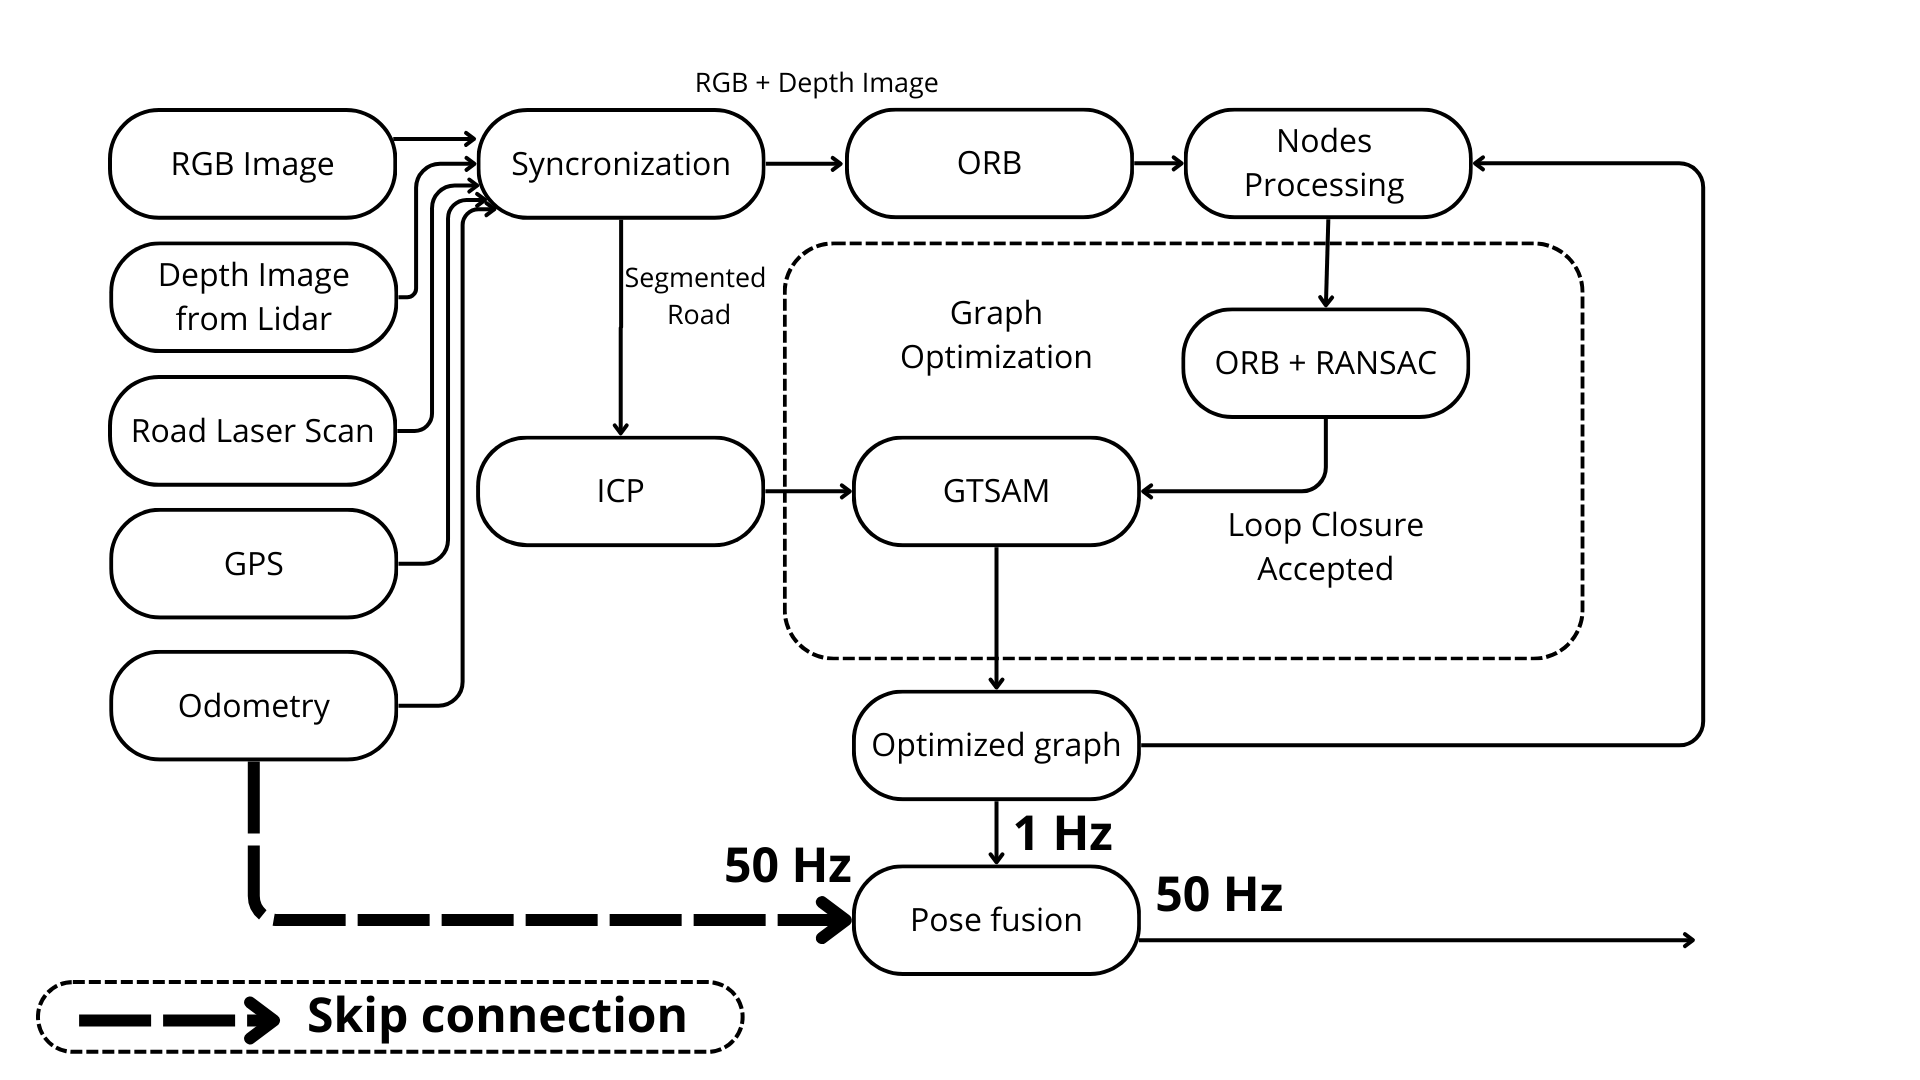
\includegraphics[width=\linewidth]{../konten/slam_arch2.png}
        \caption{Block Diagram of Graph Based SLAM based on Extended RTAB-Map \cite{ref_ku_icamimia}}
        \label{fig:graph_slam}
    \end{figure}

    Figure \ref{fig:graph_slam} is the internal explanation of SLAM block in figure \ref{fig:middleware_system}. The Graph Based SLAM is responsible for providing the best estimation of vehicle pose by fusing all sensor data from RGB image, Depth image, Road laser scan, GPS, and Odometry from wheel encoder and IMU. The Graph Based SLAM consists of several main parts, which are Synchronization, Nodes Processing, Loop Closure Detection, Graph Optimization, and Pose Fusion. 
    \par    
    The difference between our improved Graph Based SLAM with the previous Extended RTAB-Map \cite{ref_ku_icamimia} is the addition of GPS sensor to be a first guess for loop closure finding process. Another difference is doing ORB feature extraction instead of using GFTT because \cite{ref_image_matching} said that ORB better than GFTT in outdoor environment. 
}

\newcommand{\GraphBasedSLAMMode}{
    The Graph Based SLAM has two modes of operation, which are Mapping Mode and Localization Mode. In Mapping Mode, the Graph Based SLAM builds a map of the environment while simultaneously estimating the vehicle's pose. This mode is typically used during the initial exploration of an unknown environment. In Localization Mode, the Graph Based SLAM uses the previously built map to estimate the vehicle's pose without updating the map. This mode is typically used when the vehicle is operating in a known environment.
}

\newcommand{\SensorFusion}{
    The first step of Graph Based SLAM is Synchronization. Based on \cite{ref_ku_icamimia}, the synchronization strategy has been done using approximate time synchronization. The approximate time synchronization is done to synchronize all sensor data from RGB image, Depth image, Road laser scan, GPS, and Odometry from wheel encoder and IMU. The synchronized data is then used for the next step,
}

\newcommand{\NodesProcessing}{
    The first step of Nodes Processing is feature extraction of the image from camera. The feature extraction is done using ORB (Oriented FAST and Rotated BRIEF) \cite{ref_orb_ransac} to extract keypoints and descriptors from the RGB image and Depth image. After the extraction done, the Node controller will check if the current node is new or revisited node. If the current node is a new node, the node controller will add the new node to the graph. The new node will contain the RGB image, Depth image, Road laser scan, GPS, and Odometry data. If the current node is a revisited node, the node controller will proceed to the Loop Closure Detection step. 
}

\newcommand{\LoopClosureDetection}{
    After all the feature extraction has done, the next step is to find loop closure candidates. By doing first guess using GPS data (LoopGPS=true), the loop closure will only search for candidate inside LocalRadius searching area \cite{ref_rtabmap_real}. Like the method from \cite{ref_ku_icamimia}, the loop closure detection is done using feature matching between the current node and the nodes inside the LocalRadius searching area. The feature matching is done using ORB descriptors and RANSAC to filter out outliers. If the number of inliers is greater than a predefined threshold, the loop closure hypothesis is added. 
}

\newcommand{\GraphOptimization}{
    After the loop closure hypothesis has been found, the next step is Graph Optimization. The graph optimization is done using GTSAM (Georgia Tech Smoothing and Mapping) \cite{ref_gtsam} to optimize the graph and find the best estimation of vehicle pose by using the ICP constraint and odometry constraint. The graph optimization is done using the Levenberg-Marquardt algorithm to minimize the error between the predicted pose and the observed pose from the sensor data. The optimized graph is then used for the next step, which is Pose Fusion.
}

\newcommand{\PoseFusion}{
    Like the method from \cite{ref_ku_icamimia}, the Pose Fusion is done using an Extended Kalman Filter (EKF) to fuse the optimized pose from the Graph Optimization step with the odometry data from the wheel encoder and IMU. The fusion strategy use an odometry data as a velocity by differentiating the position data from odometry. The pose estimation from Graph Optimization is used as a measurement for position update in EKF. The output of the Pose Fusion is the best estimation of vehicle pose, which is then used by the High Level Program Architecture for trajectory planning and control.
}

\newcommand{\HighLevelProgramArchitecture}{
    asd asd asd asd asd asd asd asd    
    lorem ipsum dolor sit amet, consectetur adipiscing elit, sed do eiusmod tempor incididunt ut labore et dolore magna aliqua. Ut enim ad minim veniam, quis nostrud exercitation ullamco laboris nisi ut aliquip ex ea commodo consequat. Duis aute irure dolor in reprehenderit in voluptate velit esse cillum dolore eu fugiat nulla pariatur. Excepteur sint occaecat cupidatat non proident, sunt in culpa qui officia deserunt mollit anim id est laborum.
}

\newcommand{\GraphBasedSLAMandMachineLearningIntegration}{
    asd asd asd asd asd asd asd asd    
    lorem ipsum dolor sit amet, consectetur adipiscing elit, sed do eiusmod tempor incididunt ut labore et dolore magna aliqua. Ut enim ad minim veniam, quis nostrud exercitation ullamco laboris nisi ut aliquip ex ea commodo consequat. Duis aute irure dolor in reprehenderit in voluptate velit esse cillum dolore eu fugiat nulla pariatur. Excepteur sint occaecat cupidatat non proident, sunt in culpa qui officia deserunt mollit anim id est laborum.
}

\newcommand{\ModelPredictionControl}{
    asd asd asd asd asd asd asd asd    
    lorem ipsum dolor sit amet, consectetur adipiscing elit, sed do eiusmod tempor incididunt ut labore et dolore magna aliqua. Ut enim ad minim veniam, quis nostrud exercitation ullamco laboris nisi ut aliquip ex ea commodo consequat. Duis aute irure dolor in reprehenderit in voluptate velit esse cillum dolore eu fugiat nulla pariatur. Excepteur sint occaecat cupidatat non proident, sunt in culpa qui officia deserunt mollit anim id est laborum.
}

\newcommand{\TrajectoryOptimization}{
    asd asd asd asd asd asd asd asd    
    lorem ipsum dolor sit amet, consectetur adipiscing elit, sed do eiusmod tempor incididunt ut labore et dolore magna aliqua. Ut enim ad minim veniam, quis nostrud exercitation ullamco laboris nisi ut aliquip ex ea commodo consequat. Duis aute irure dolor in reprehenderit in voluptate velit esse cillum dolore eu fugiat nulla pariatur. Excepteur sint occaecat cupidatat non proident, sunt in culpa qui officia deserunt mollit anim id est laborum.
}

\newcommand{\TargetVelocityandSteeringCalculation}{
    asd asd asd asd asd asd asd asd    
    lorem ipsum dolor sit amet, consectetur adipiscing elit, sed do eiusmod tempor incididunt ut labore et dolore magna aliqua. Ut enim ad minim veniam, quis nostrud exercitation ullamco laboris nisi ut aliquip ex ea commodo consequat. Duis aute irure dolor in reprehenderit in voluptate velit esse cillum dolore eu fugiat nulla pariatur. Excepteur sint occaecat cupidatat non proident, sunt in culpa qui officia deserunt mollit anim id est laborum.
}

\newcommand{\SafetySystem}{
    asd asd asd asd asd asd asd asd    
    lorem ipsum dolor sit amet, consectetur adipiscing elit, sed do eiusmod tempor incididunt ut labore et dolore magna aliqua. Ut enim ad minim veniam, quis nostrud exercitation ullamco laboris nisi ut aliquip ex ea commodo consequat. Duis aute irure dolor in reprehenderit in voluptate velit esse cillum dolore eu fugiat nulla pariatur. Excepteur sint occaecat cupidatat non proident, sunt in culpa qui officia deserunt mollit anim id est laborum.
}

\newcommand{\ISOImplementation}{
    asd asd asd asd asd asd asd asd    
    lorem ipsum dolor sit amet, consectetur adipiscing elit, sed do eiusmod tempor incididunt ut labore et dolore magna aliqua. Ut enim ad minim veniam, quis nostrud exercitation ullamco laboris nisi ut aliquip ex ea commodo consequat. Duis aute irure dolor in reprehenderit in voluptate velit esse cillum dolore eu fugiat nulla pariatur. Excepteur sint occaecat cupidatat non proident, sunt in culpa qui officia deserunt mollit anim id est laborum.
}

\newcommand{\EmergencyStopSystem}{
    asd asd asd asd asd asd asd asd    
    lorem ipsum dolor sit amet, consectetur adipiscing elit, sed do eiusmod tempor incididunt ut labore et dolore magna aliqua. Ut enim ad minim veniam, quis nostrud exercitation ullamco laboris nisi ut aliquip ex ea commodo consequat. Duis aute irure dolor in reprehenderit in voluptate velit esse cillum dolore eu fugiat nulla pariatur. Excepteur sint occaecat cupidatat non proident, sunt in culpa qui officia deserunt mollit anim id est laborum.
}

\newcommand{\SafetyTests}{
    asd asd asd asd asd asd asd asd    
    lorem ipsum dolor sit amet, consectetur adipiscing elit, sed do eiusmod tempor incididunt ut labore et dolore magna aliqua. Ut enim ad minim veniam, quis nostrud exercitation ullamco laboris nisi ut aliquip ex ea commodo consequat. Duis aute irure dolor in reprehenderit in voluptate velit esse cillum dolore eu fugiat nulla pariatur. Excepteur sint occaecat cupidatat non proident, sunt in culpa qui officia deserunt mollit anim id est laborum.
}
